\documentclass{sjtuarticle}

\usepackage[perpage,bottom,hang]{footmisc}
\usepackage[ruled,vlined,linesnumbered]{algorithm2e}
\usepackage{listings}
\lstdefinestyle{lstStyleCode}{
  basicstyle=\ttfamily\footnotesize,
  breaklines=true,
  showstringspaces=false,
  showspaces=false,
  mathescape=false,
  frame=single,
  numbers=left,
  numberstyle=\tiny,
  tabsize=4,
  columns=flexible
}
\lstnewenvironment{codeblock}[1][]%
  {\lstset{style=lstStyleCode,#1}}{}
\usepackage{booktabs}
\usepackage{longtable}
\usepackage{threeparttable}
\usepackage{threeparttablex}
\usepackage{hyperref}
\usepackage{multicol}
\usepackage{multirow}
\usepackage{graphicx}
\usepackage{float}

\graphicspath{{images/}}
\setlength{\textfloatsep}{8pt plus 2pt minus 2pt}
\setlength{\floatsep}{8pt plus 2pt minus 2pt}
\setlength{\intextsep}{8pt plus 2pt minus 2pt}

\title{realtimeshadow 报告}
\author{安燕杰  \and  李志阳}

\begin{document}
\maketitle

\begin{abstract}
本文基于 WebGL 实现 Two-Pass Shadow Map、PCF 和 PCSS，并扩展了 blocker 调试可视化、多光源叠加、移动光源和动态模型。实现中每个光源独立生成 Shadow Map，在 camera pass 中进行深度比较；PCF 使用 Poisson 圆盘多采样，PCSS 在此基础上加入 blocker search 和动态半影估计。实验对比了硬阴影、PCF 与 PCSS 的结果，三种模式可通过 GUI 下拉菜单运行时切换。
\end{abstract}

\section{问题背景}

实时阴影用于表达光源、遮挡物和接收面的空间关系。局部光照模型只能计算表面明暗，不能处理物体间遮挡；而离线路径追踪代价过高，不适合 WebGL 实时场景。因此本项目采用 Shadow Map：先从光源视角记录最近深度，再在相机视角比较当前片元深度与 Shadow Map 深度。

基础 Shadow Map 得到的是硬阴影，边缘容易锯齿，也不能表达面积光产生的半影。PCF 通过多次深度测试并求平均柔化边缘；PCSS 进一步搜索 blocker 平均深度，按接收面与遮挡物的距离动态调整滤波半径。

\section{研究内容与方法}

\subsection{整体渲染流程}

渲染采用 Two-Pass Shadow Map。Shadow Pass 从当前光源视角将深度写入该光源的 FBO；Camera Pass 从相机视角绘制模型，并在片元着色器中采样对应 Shadow Map 完成遮挡判断。普通网格保存在 \texttt{renderer.meshes}，阴影网格按光源索引保存在 \texttt{renderer.shadowMeshes[lightIndex]}。渲染器逐个遍历光源，每个光源独立生成 Shadow Map 并绘制一次 camera pass；第二个及后续光源只叠加直接光照。

\subsection{光源空间矩阵与 Shadow Map}

为了将模型顶点变换到光源视角，需要计算光源 MVP 矩阵：

\[
MVP_{light}=P_{light}V_{light}M
\]

模型矩阵由平移和缩放构成，视图矩阵由 \texttt{lookAt(lightPos, focalPoint, lightUp)} 构成。方向光使用正交投影，范围为 \([-120,120]\times[-70,110]\)，近远平面为 \(40,240\)。主光源位于 \((0,80,80)\)，第二个光源在 XZ 平面轨道运动，二者均看向场景中心。

Shadow Pass 将 \texttt{gl\_FragCoord.z} 打包到 RGBA 纹理；Camera Pass 通过 \texttt{unpack()} 还原深度。该方式避免了 WebGL1 中直接依赖深度纹理的兼容性问题。

\subsection{硬阴影实现}

硬阴影由 \texttt{useShadowMap()} 完成。片元将 \texttt{vPositionFromLight} 从 NDC 映射到 \([0,1]\)，然后比较当前深度与 Shadow Map 中记录的最近深度：

\[
visibility =
\begin{cases}
0, & z_{receiver}-bias > z_{shadow} \\
1, & otherwise
\end{cases}
\]

当前使用 \texttt{SHADOW\_BIAS = 0.012} 缓解多光源叠加下的 shadow acne；投影坐标超出 Shadow Map 范围时直接认为可见。

\subsection{PCF 软阴影实现}

PCF 在片元周围做多次 shadow test 并取平均：

\[
visibility = \frac{1}{N}\sum_{i=1}^{N} shadowTest(uv + offset_i \cdot r)
\]

采样核使用 Poisson 圆盘，采样数为 40，固定滤波半径为 \texttt{PCF\_FILTER\_SIZE = 0.0035}。代码中将固定半径 PCF 抽成 \texttt{PCFWithFilterSize()}，供普通 PCF 和 PCSS 的动态半径滤波共同调用。Shadow Map 纹理设置为 \texttt{CLAMP\_TO\_EDGE}，shader 中也对每个 \texttt{sampleUV} 做边界检查。

\subsection{PCSS 软阴影实现}

PCSS 在 PCF 前加入遮挡物搜索和半影估计。\texttt{findBlocker()} 在当前 UV 附近搜索比接收点更靠近光源的样本：

\[
z_{receiver} - bias > z_{sample}
\]

满足条件的样本视为 blocker，累加后取平均得到 \texttt{avgBlockerDepth}；若没有 blocker，则该片元直接可见。

PCSS 根据接收点和 blocker 的深度差估算半影：

\[
penumbraRatio=\frac{z_{receiver}-z_{blocker}}{\max(z_{blocker},\epsilon)}
\]

该比例乘以 \texttt{LIGHT\_SIZE\_UV} 得到动态滤波半径，并限制在 \([0.0008,0.009]\) 范围内，最后调用 \texttt{PCFWithFilterSize()}。因此当前 PCSS 的实际流程为：blocker 搜索、半影半径估计、动态半径 PCF。

\subsection{光照合成方式}

阴影只衰减直接光照，不压暗环境光。片元颜色使用
\[
radiance=uApplyAmbient\cdot ambient+visibility\cdot(diffuse+specular)
\]
计算，多光源渲染中只有第一个光源 pass 加入 ambient，后续 pass 设置 \texttt{uApplyAmbient = 0.0}，避免重复累加环境光。

\subsection{调试可视化}

调试开关由 dat.gui 控制。\texttt{Show Shadow Map} 在右下角叠加 Shadow Map 灰度图；\texttt{Show Blocker Search} 复用 blocker 搜索逻辑统计邻域遮挡样本比例，并用绿色到红色映射 blocker 密度。

\subsection{多光源与移动光源}

额外任务使用两个方向光：Light 0 为固定暖色主光，位置 \((0,80,80)\)，强度 3000；Light 1 为轨道运动冷色光，初始位置 \((80,70,0)\)，强度 2500。每个光源都有独立的 \(8192 \times 8192\) Shadow Map FBO。移动光源按 \(x=\cos(t\cdot0.0005)\cdot100,\ z=\sin(t\cdot0.0005)\cdot100\) 更新位置；位置变化后，渲染器重新计算 \texttt{uLightMVP} 并同步相关 uniform。

额外任务还实现了场景中的动态模型。Mary 模型的 transform 添加了 \texttt{rotation} 属性，模型矩阵由原来的 \(T \times S\) 扩展为 \(T \times R \times S\)。小 Mary（缩放 10 倍，含身体和 "202" 徽标两个子 mesh）在 XZ 平面做圆形轨道运动（半径 25），同时绕 Y 轴自转。两个子 mesh 的 transform 分别存储在数组中，动画循环统一更新，确保 "202" 徽标始终附着在模型胸部。阴影 pass 与相机 pass 共享 transform，因此阴影正确跟随模型移动。

\subsection{主要参数}

\begin{table}[htbp]
\centering
\caption{当前实现使用的主要参数}
\begin{tabular}{lll}
\toprule
参数 & 当前值 & 作用 \\
\midrule
Shadow Map 分辨率 & \(8192 \times 8192\) & 提高阴影采样精度 \\
Light 0 & 强度 3000，颜色 \((1.0,0.95,0.9)\)，位置 \((0,80,80)\) & 固定暖色主光 \\
Light 1 & 强度 2500，颜色 \((0.7,0.8,1.0)\)，初始位置 \((80,70,0)\) & 轨道运动冷色光 \\
光源正交投影 & \([-120,120],[-70,110],40,240\) & 覆盖当前场景并控制深度精度 \\
\texttt{NUM\_SAMPLES} & 40 & PCF 与 PCSS 的采样数 \\
\texttt{SHADOW\_BIAS} & 0.012 & 缓解多光源叠加下的 shadow acne \\
\texttt{PCF\_FILTER\_SIZE} & 0.0035 & PCF 固定滤波半径 \\
\texttt{BLOCKER\_SEARCH\_SIZE} & 0.0045 & PCSS blocker 搜索半径 \\
\texttt{LIGHT\_SIZE\_UV} & 0.007 & 模拟面积光大小 \\
\texttt{PCSS\_MIN\_FILTER\_SIZE} & 0.0008 & PCSS 最小滤波半径 \\
\texttt{PCSS\_MAX\_FILTER\_SIZE} & 0.009 & PCSS 最大滤波半径 \\
\bottomrule
\end{tabular}
\end{table}

\section{实验结果与分析}

实验场景由两个 Mary 模型和地板组成，包含固定暖色主光和轨道运动冷色光。实验分别截取硬阴影、PCF 和 PCSS 三种模式，并在同一场景中观察 Shadow Map 小窗、blocker 搜索可视化和双光源阴影。

\subsection{硬阴影结果}

\begin{figure}[htbp]
  \centering
  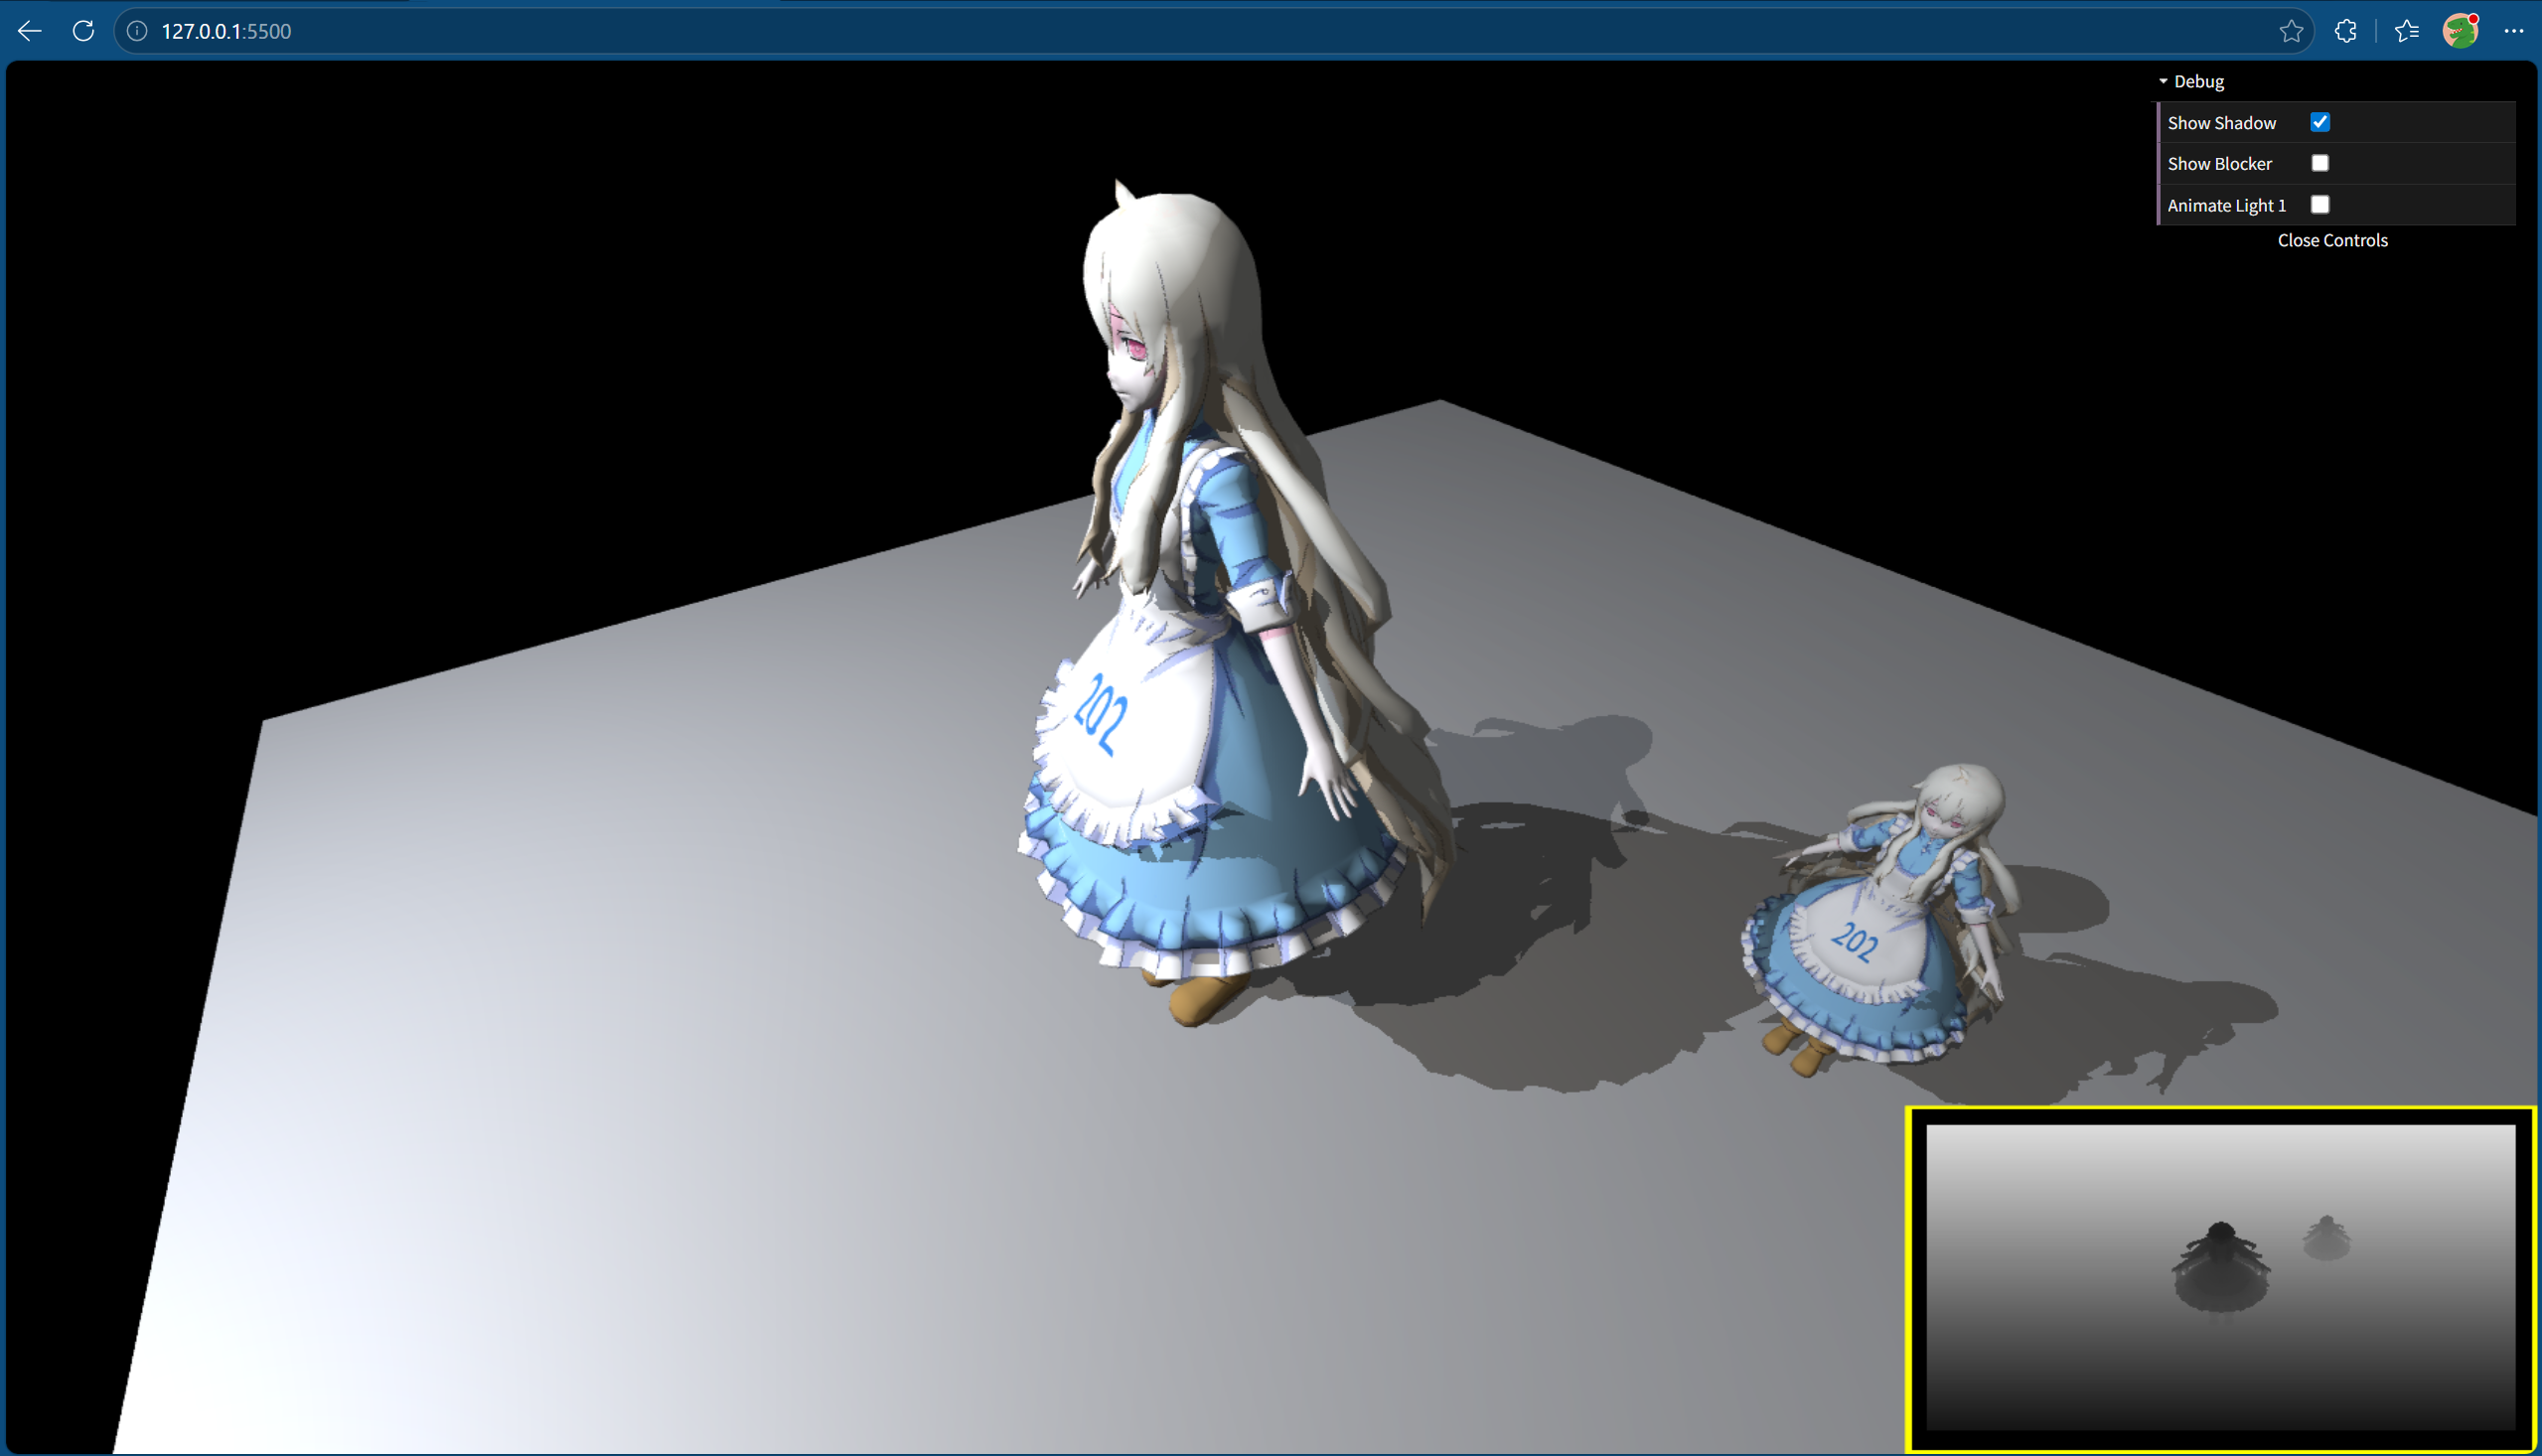
\includegraphics[width=0.76\linewidth]{SM_shadow.png}
  \caption{Shadow Map 硬阴影结果（双光源场景，右下角含 Shadow Map 小窗）}
  \label{fig:sm}
\end{figure}

图 \ref{fig:sm} 中物体在地板上形成明确阴影，说明光源 MVP、Shadow Pass、深度打包与深度比较均已正常工作。地面上两个方向的阴影来自两个独立光源，是多光源叠加的预期结果；右下角小窗为 Shadow Map 灰度可视化。硬阴影只做一次深度比较，边界为二值变化，因此轮廓处较硬且容易出现锯齿。

\subsection{PCF 结果}

\begin{figure}[htbp]
  \centering
  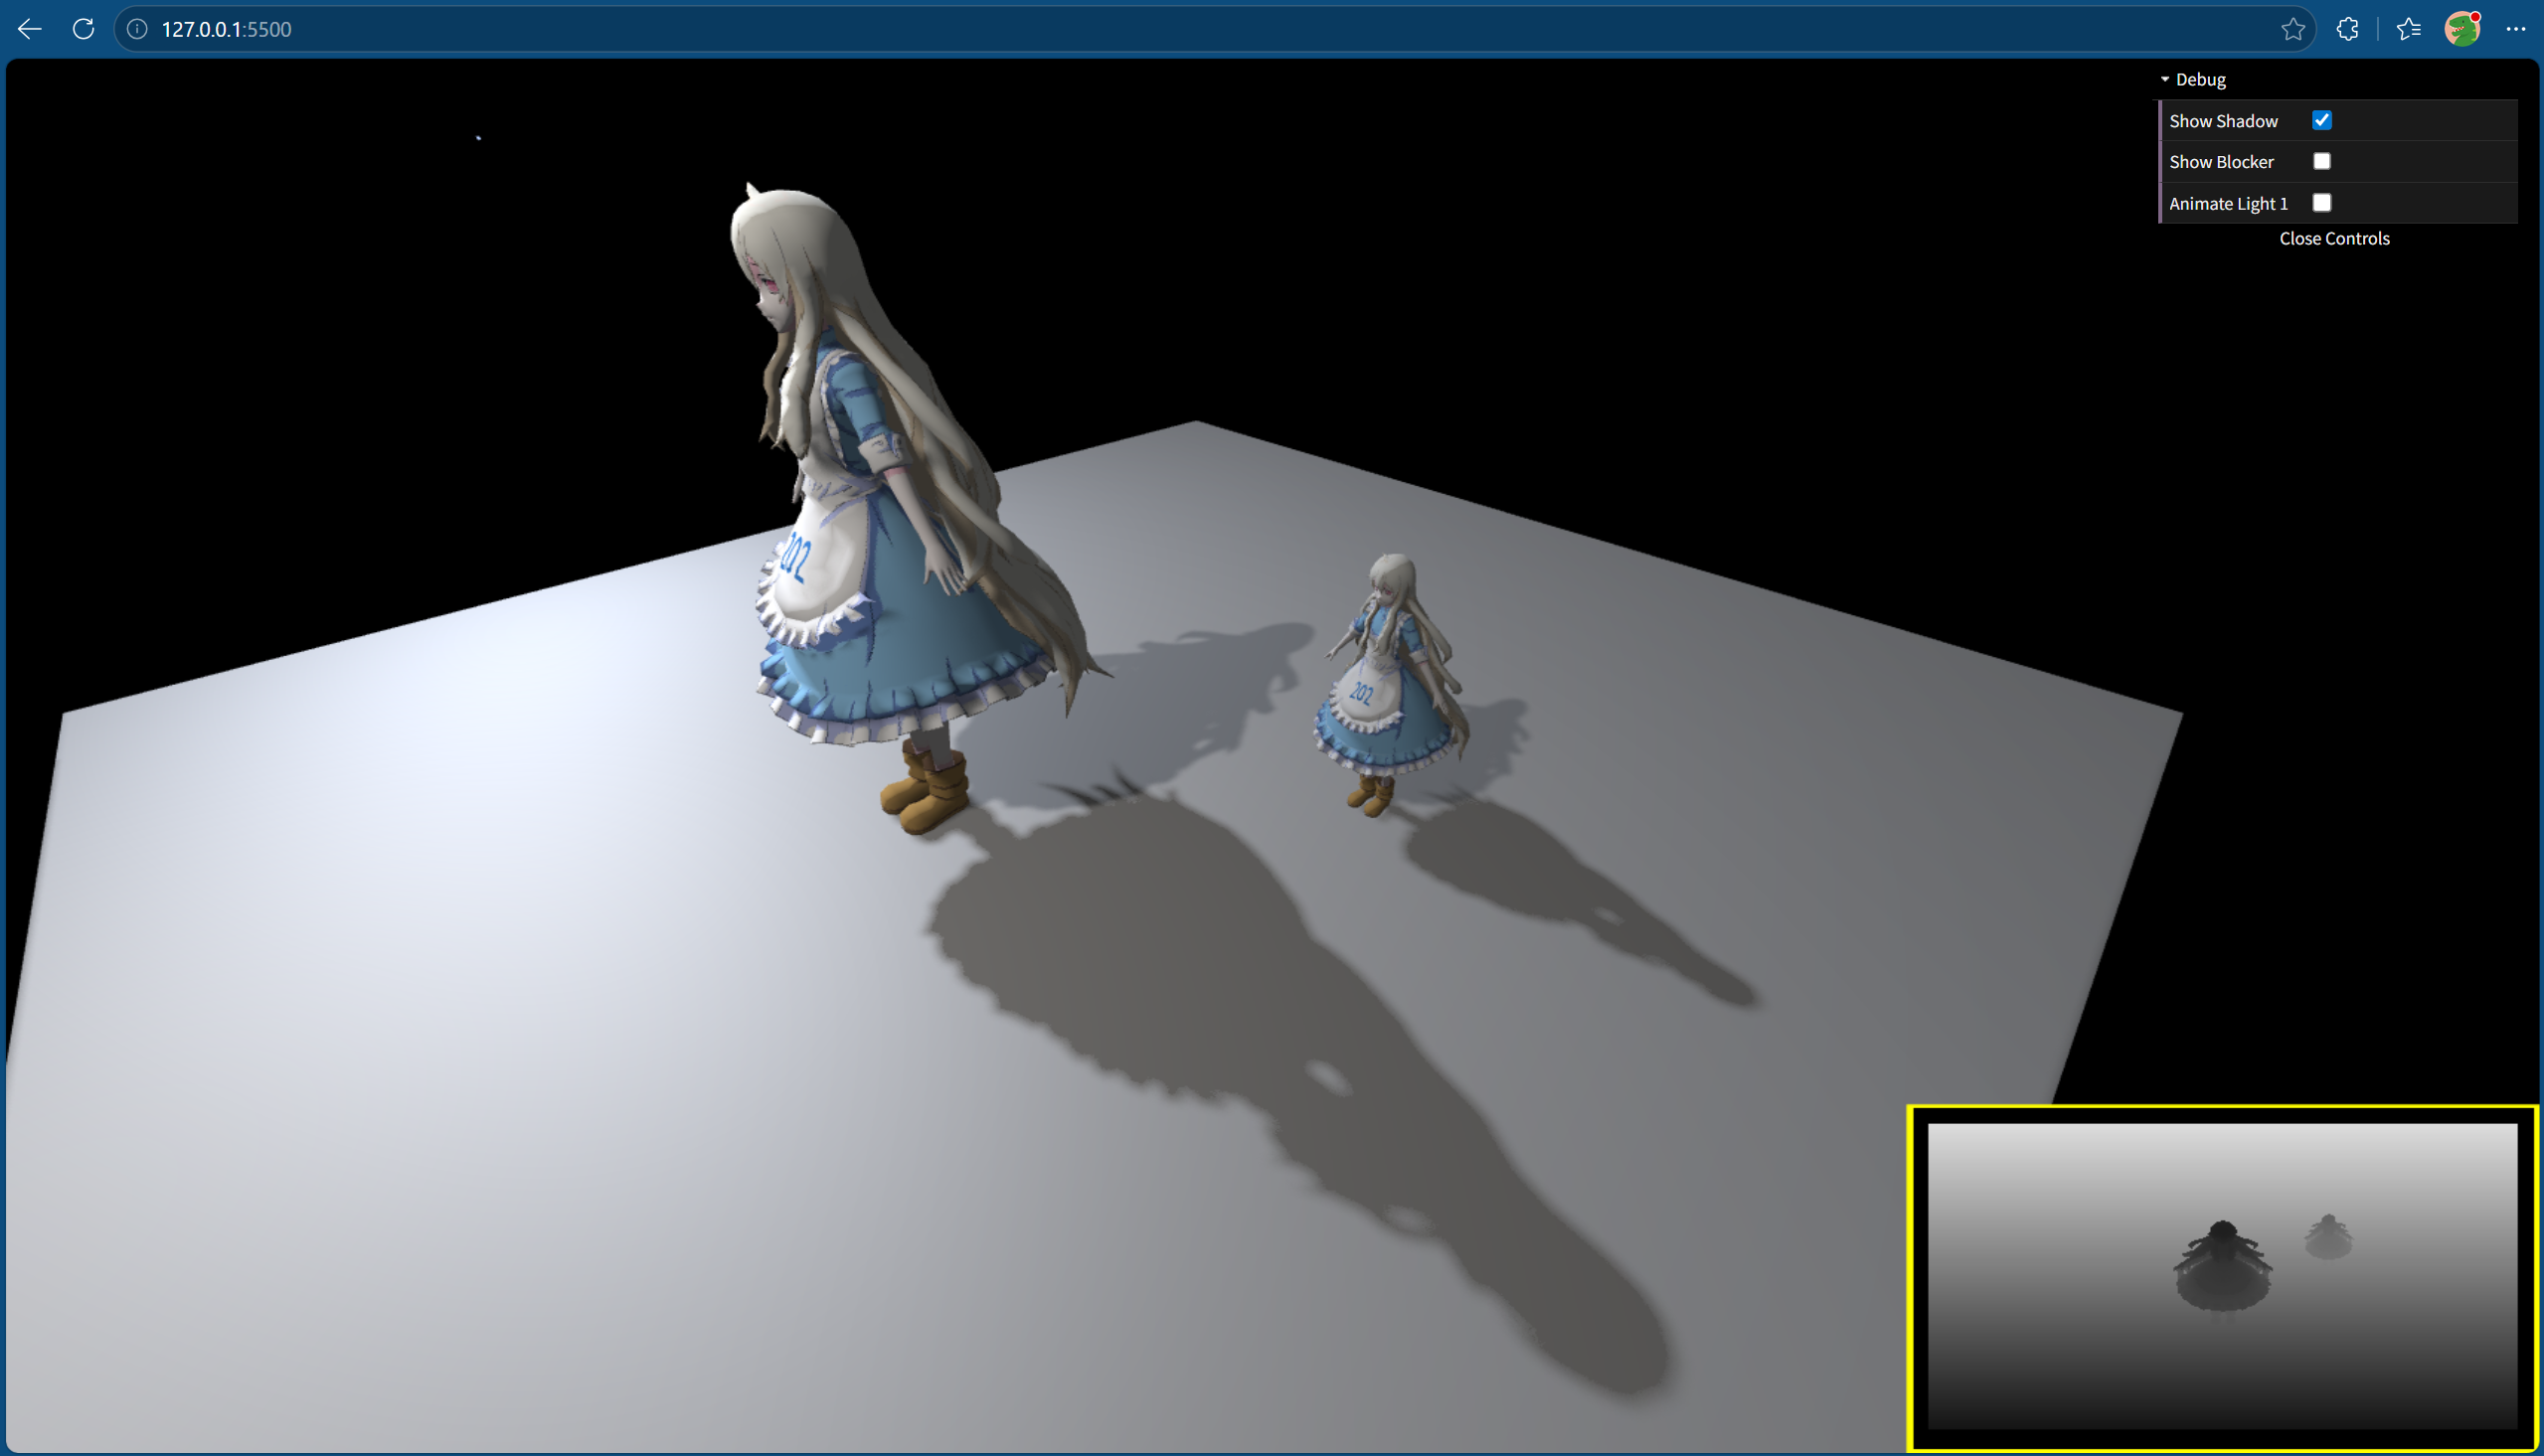
\includegraphics[width=0.76\linewidth]{PCF_shadow.png}
  \caption{PCF 软阴影结果（双光源场景，右下角含 Shadow Map 小窗）}
  \label{fig:pcf}
\end{figure}

图 \ref{fig:pcf} 展示固定半径 PCF 结果。PCF 对邻域内多次 shadow test 取平均，明显削弱硬阴影锯齿，使边缘变为连续过渡。但滤波半径固定，阴影软硬程度不随遮挡物和接收面的距离变化，接触区域与远离区域的边缘宽度差异不明显。

\subsection{PCSS 结果}

\begin{figure}[htbp]
  \centering
  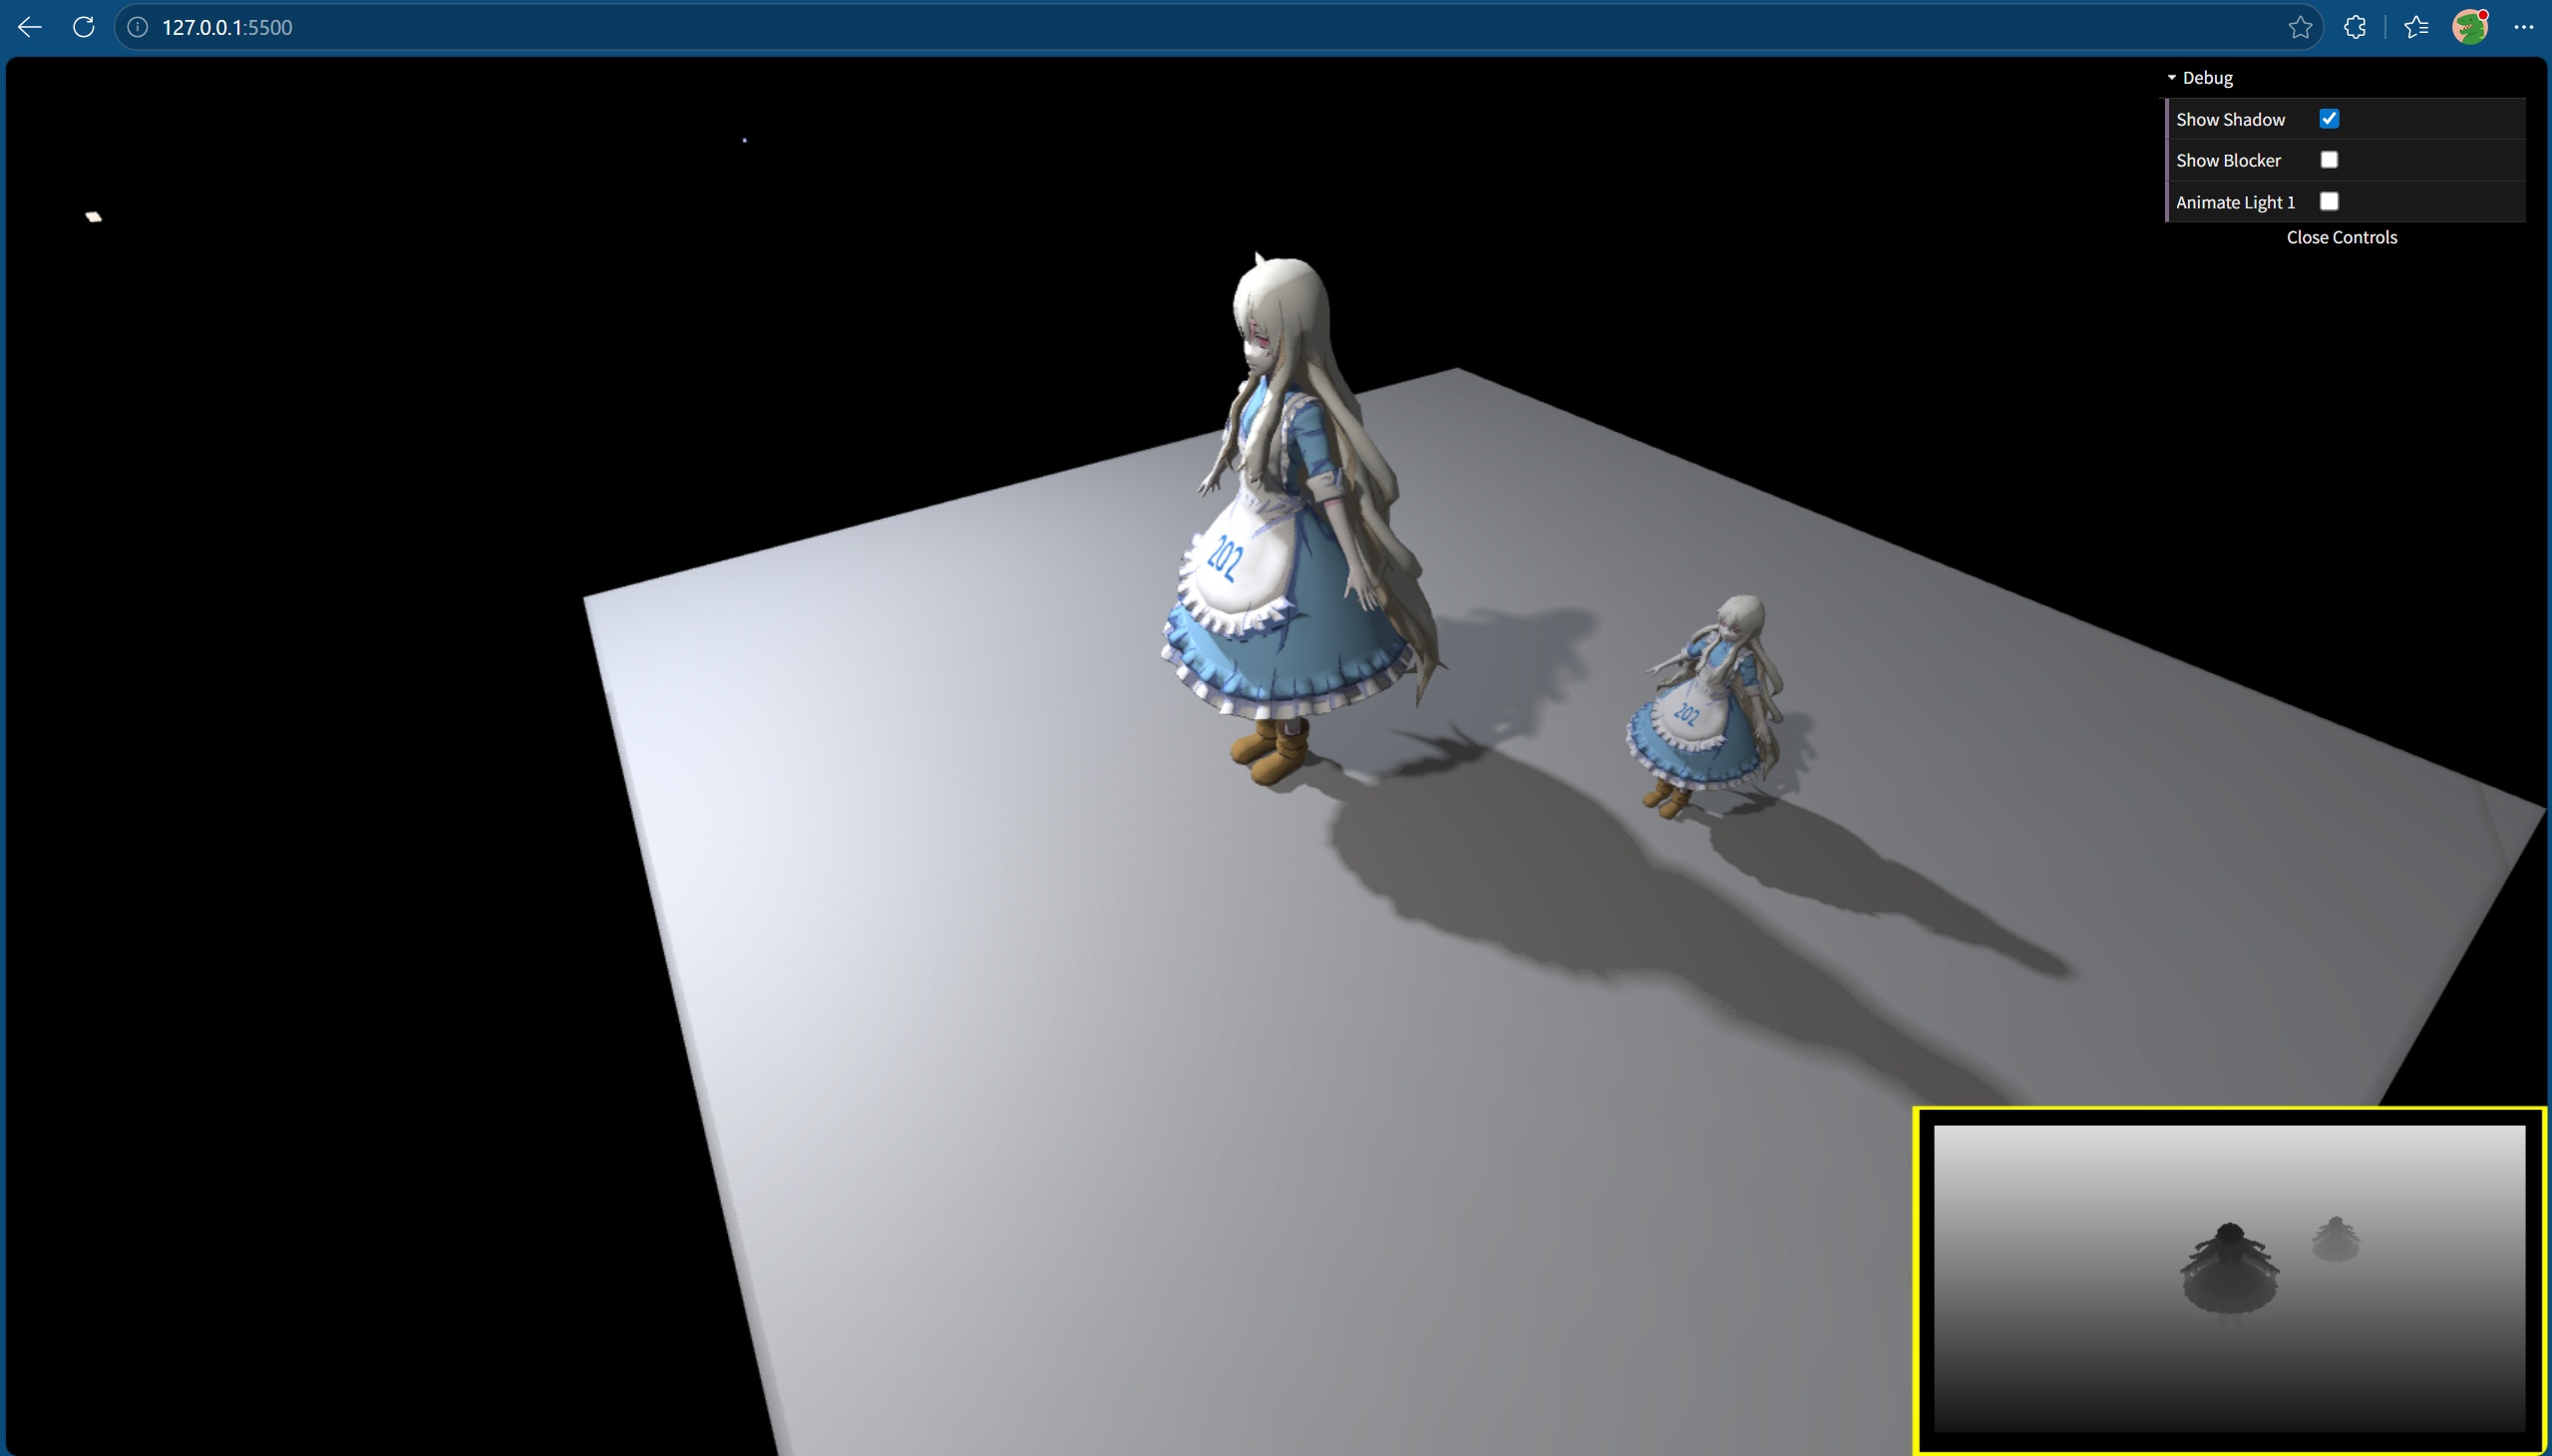
\includegraphics[width=0.76\linewidth]{PCSS_shadow.png}
  \caption{PCSS 软阴影结果（双光源场景，右下角含 Shadow Map 小窗）}
  \label{fig:pcss}
\end{figure}

图 \ref{fig:pcss} 展示 PCSS 结果。PCSS 先搜索 blocker 平均深度，再由 receiver 与 blocker 的深度差估计半影大小。相比固定半径 PCF，PCSS 能保留较清晰的接触阴影，并在距离遮挡物更远处增大滤波半径，得到更宽的边缘过渡。图中两个方向的阴影同样来自双光源叠加。

PCSS 对采样数和参数更敏感。采样过少会在复杂轮廓处产生颗粒感，采样过多会明显拖慢 WebGL 刷新和截图；当前使用 40 次采样折中质量与性能。\texttt{LIGHT\_SIZE\_UV} 和 \texttt{PCSS\_MAX\_FILTER\_SIZE} 过大会导致过度模糊，\texttt{SHADOW\_BIAS} 过小或过大则分别引入 shadow acne 或 Peter Panning。

\subsection{调试可视化结果}

Shadow Map 可视化用于确认光源视角下的深度分布是否正常。开启后，右下角小窗显示 Shadow Map 灰度图，如果出现全黑、全白或明显裁剪，通常说明 FBO 写入、光源投影范围或 lightMVP 计算存在问题。该小窗已经包含在图 \ref{fig:sm}、图 \ref{fig:pcf} 和图 \ref{fig:pcss} 中，因此不再单独放置额外截图。

Blocker 搜索可视化用于观察当前片元附近的遮挡物分布：绿色表示几乎没有 blocker，红色表示 blocker 比例较高，黄橙色表示部分遮挡。虽然 blocker search 主要服务于 PCSS，但同一套红绿色标可以叠加在硬阴影、PCF 和 PCSS 三种显示模式上，便于确认三种模式使用的是一致的遮挡关系。图 \ref{fig:blocker-debug} 给出三种模式下的结果。

\begin{figure}[htbp]
  \centering
  \begin{minipage}{0.32\linewidth}
    \centering
    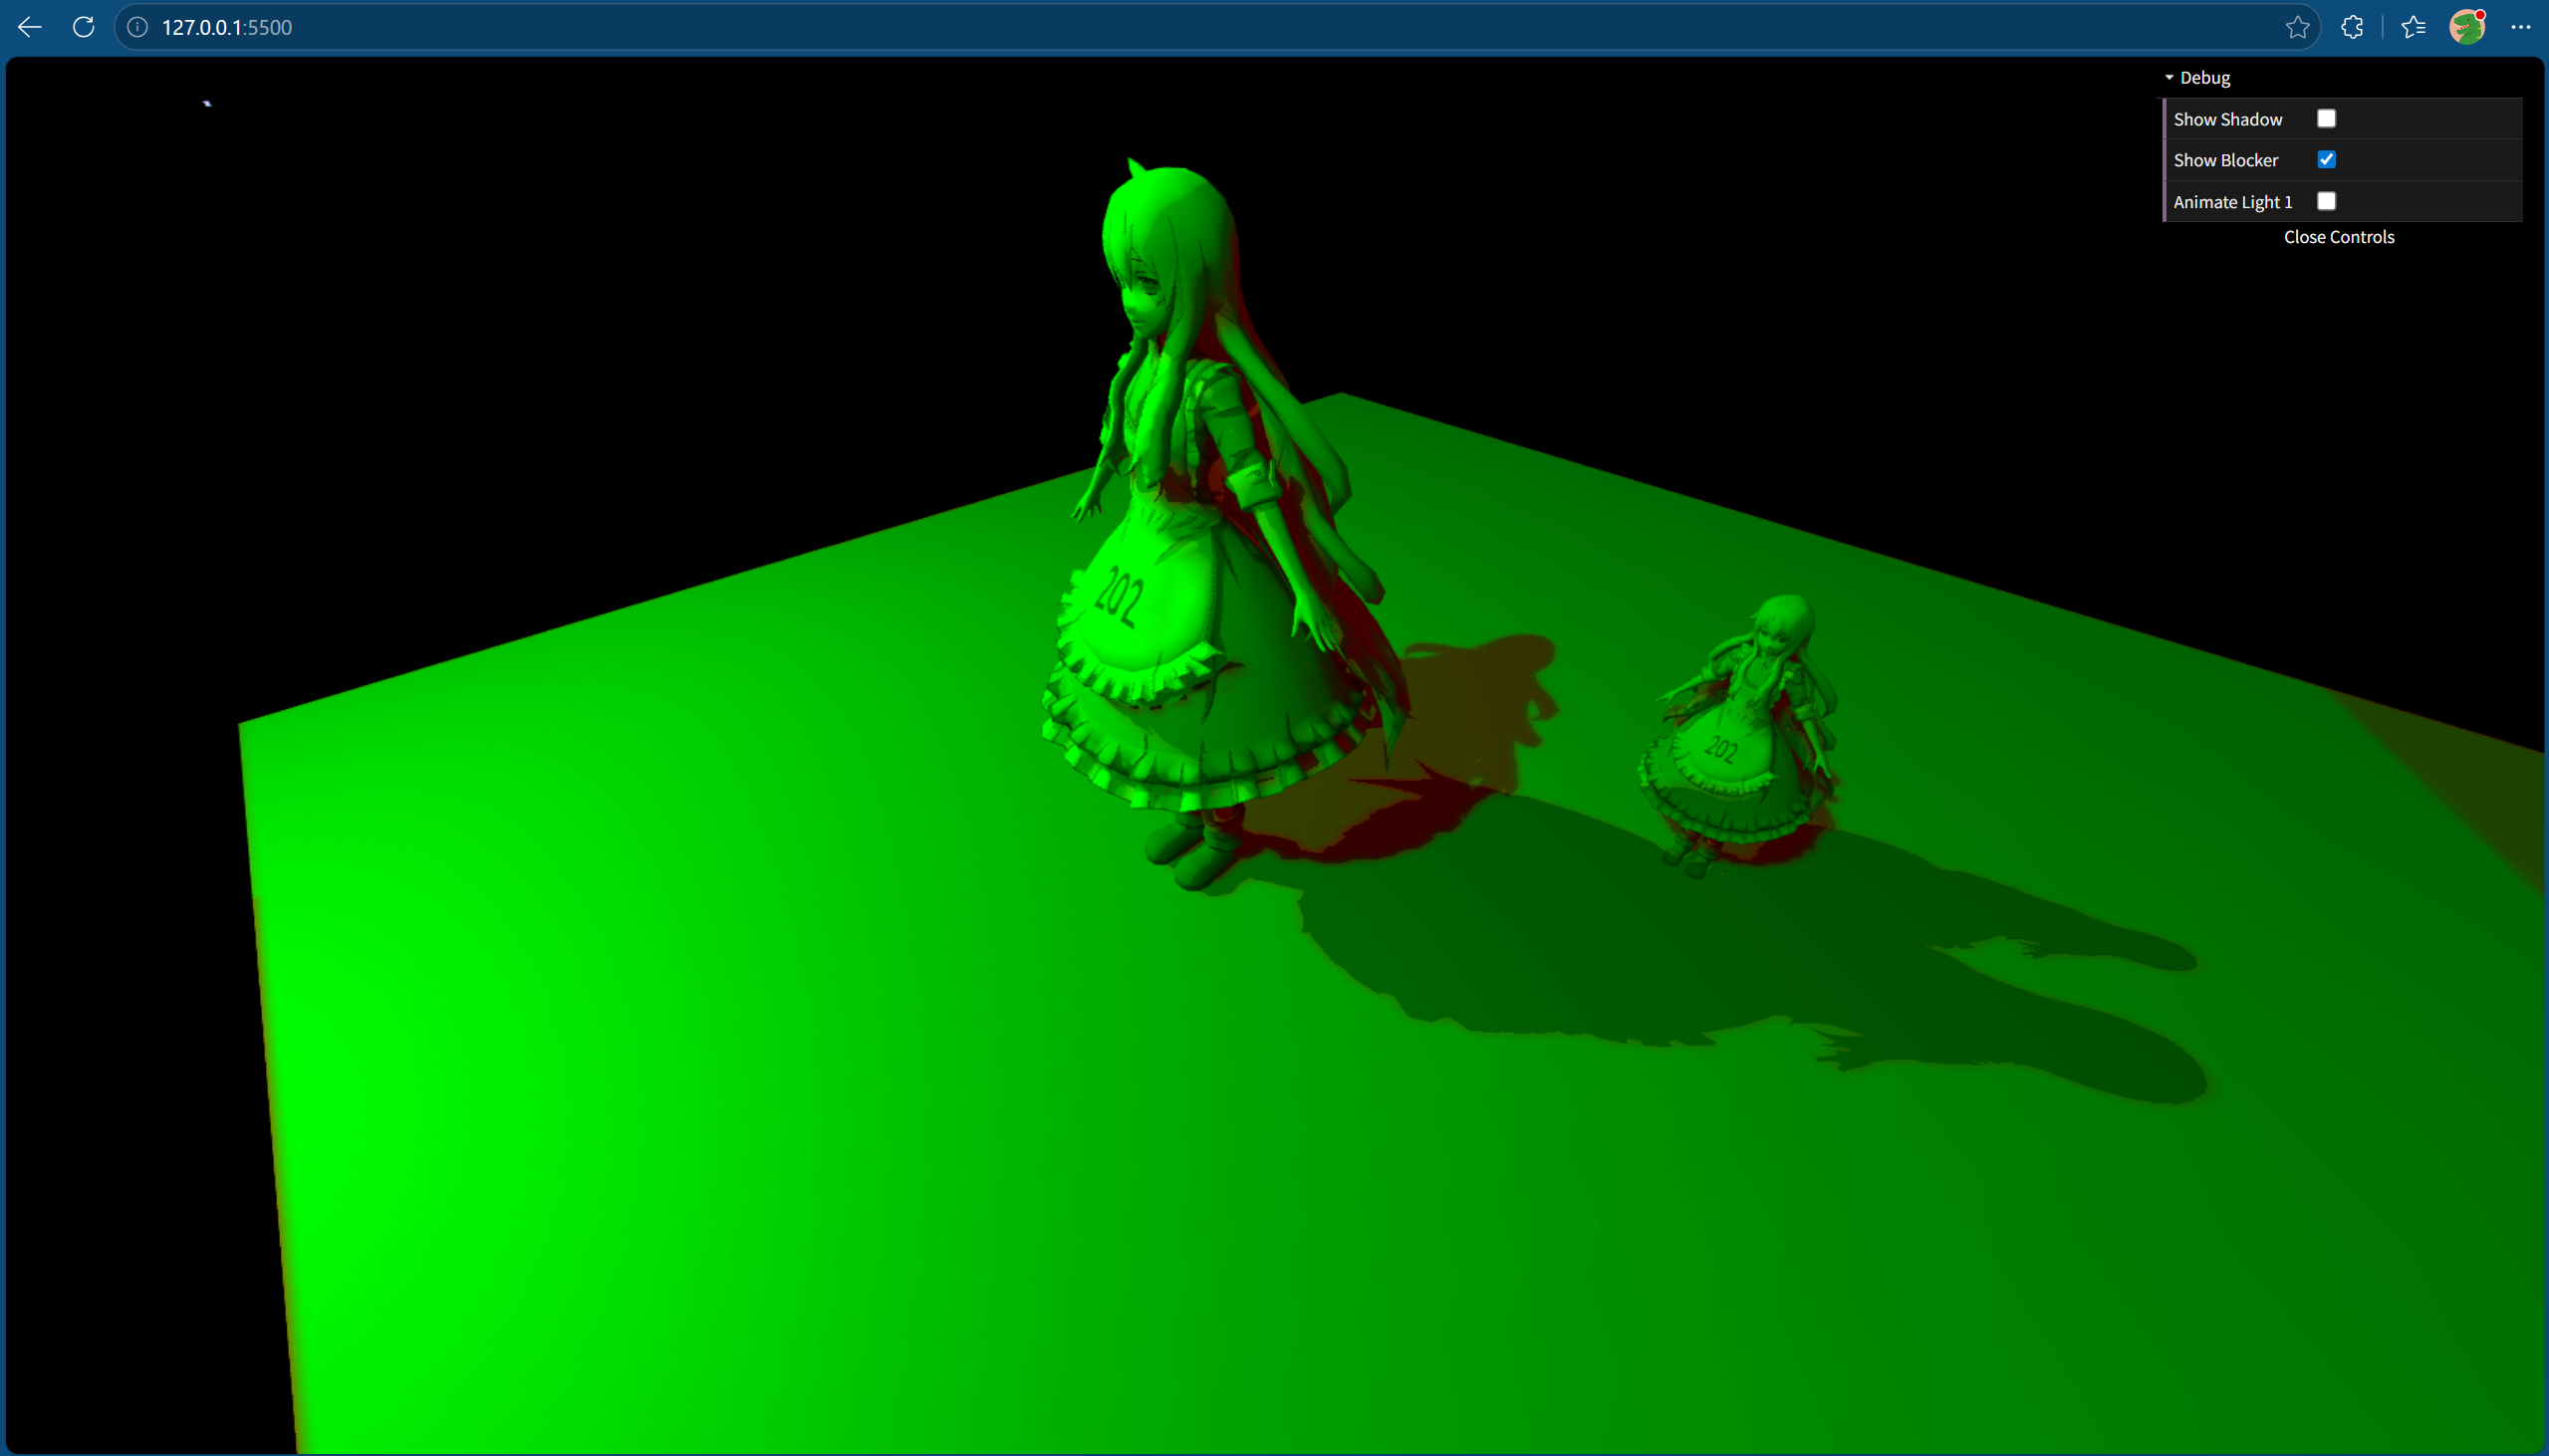
\includegraphics[width=\linewidth]{SM_blocker_debug.png}\\[-1pt]
    \small 硬阴影
  \end{minipage}
  \begin{minipage}{0.32\linewidth}
    \centering
    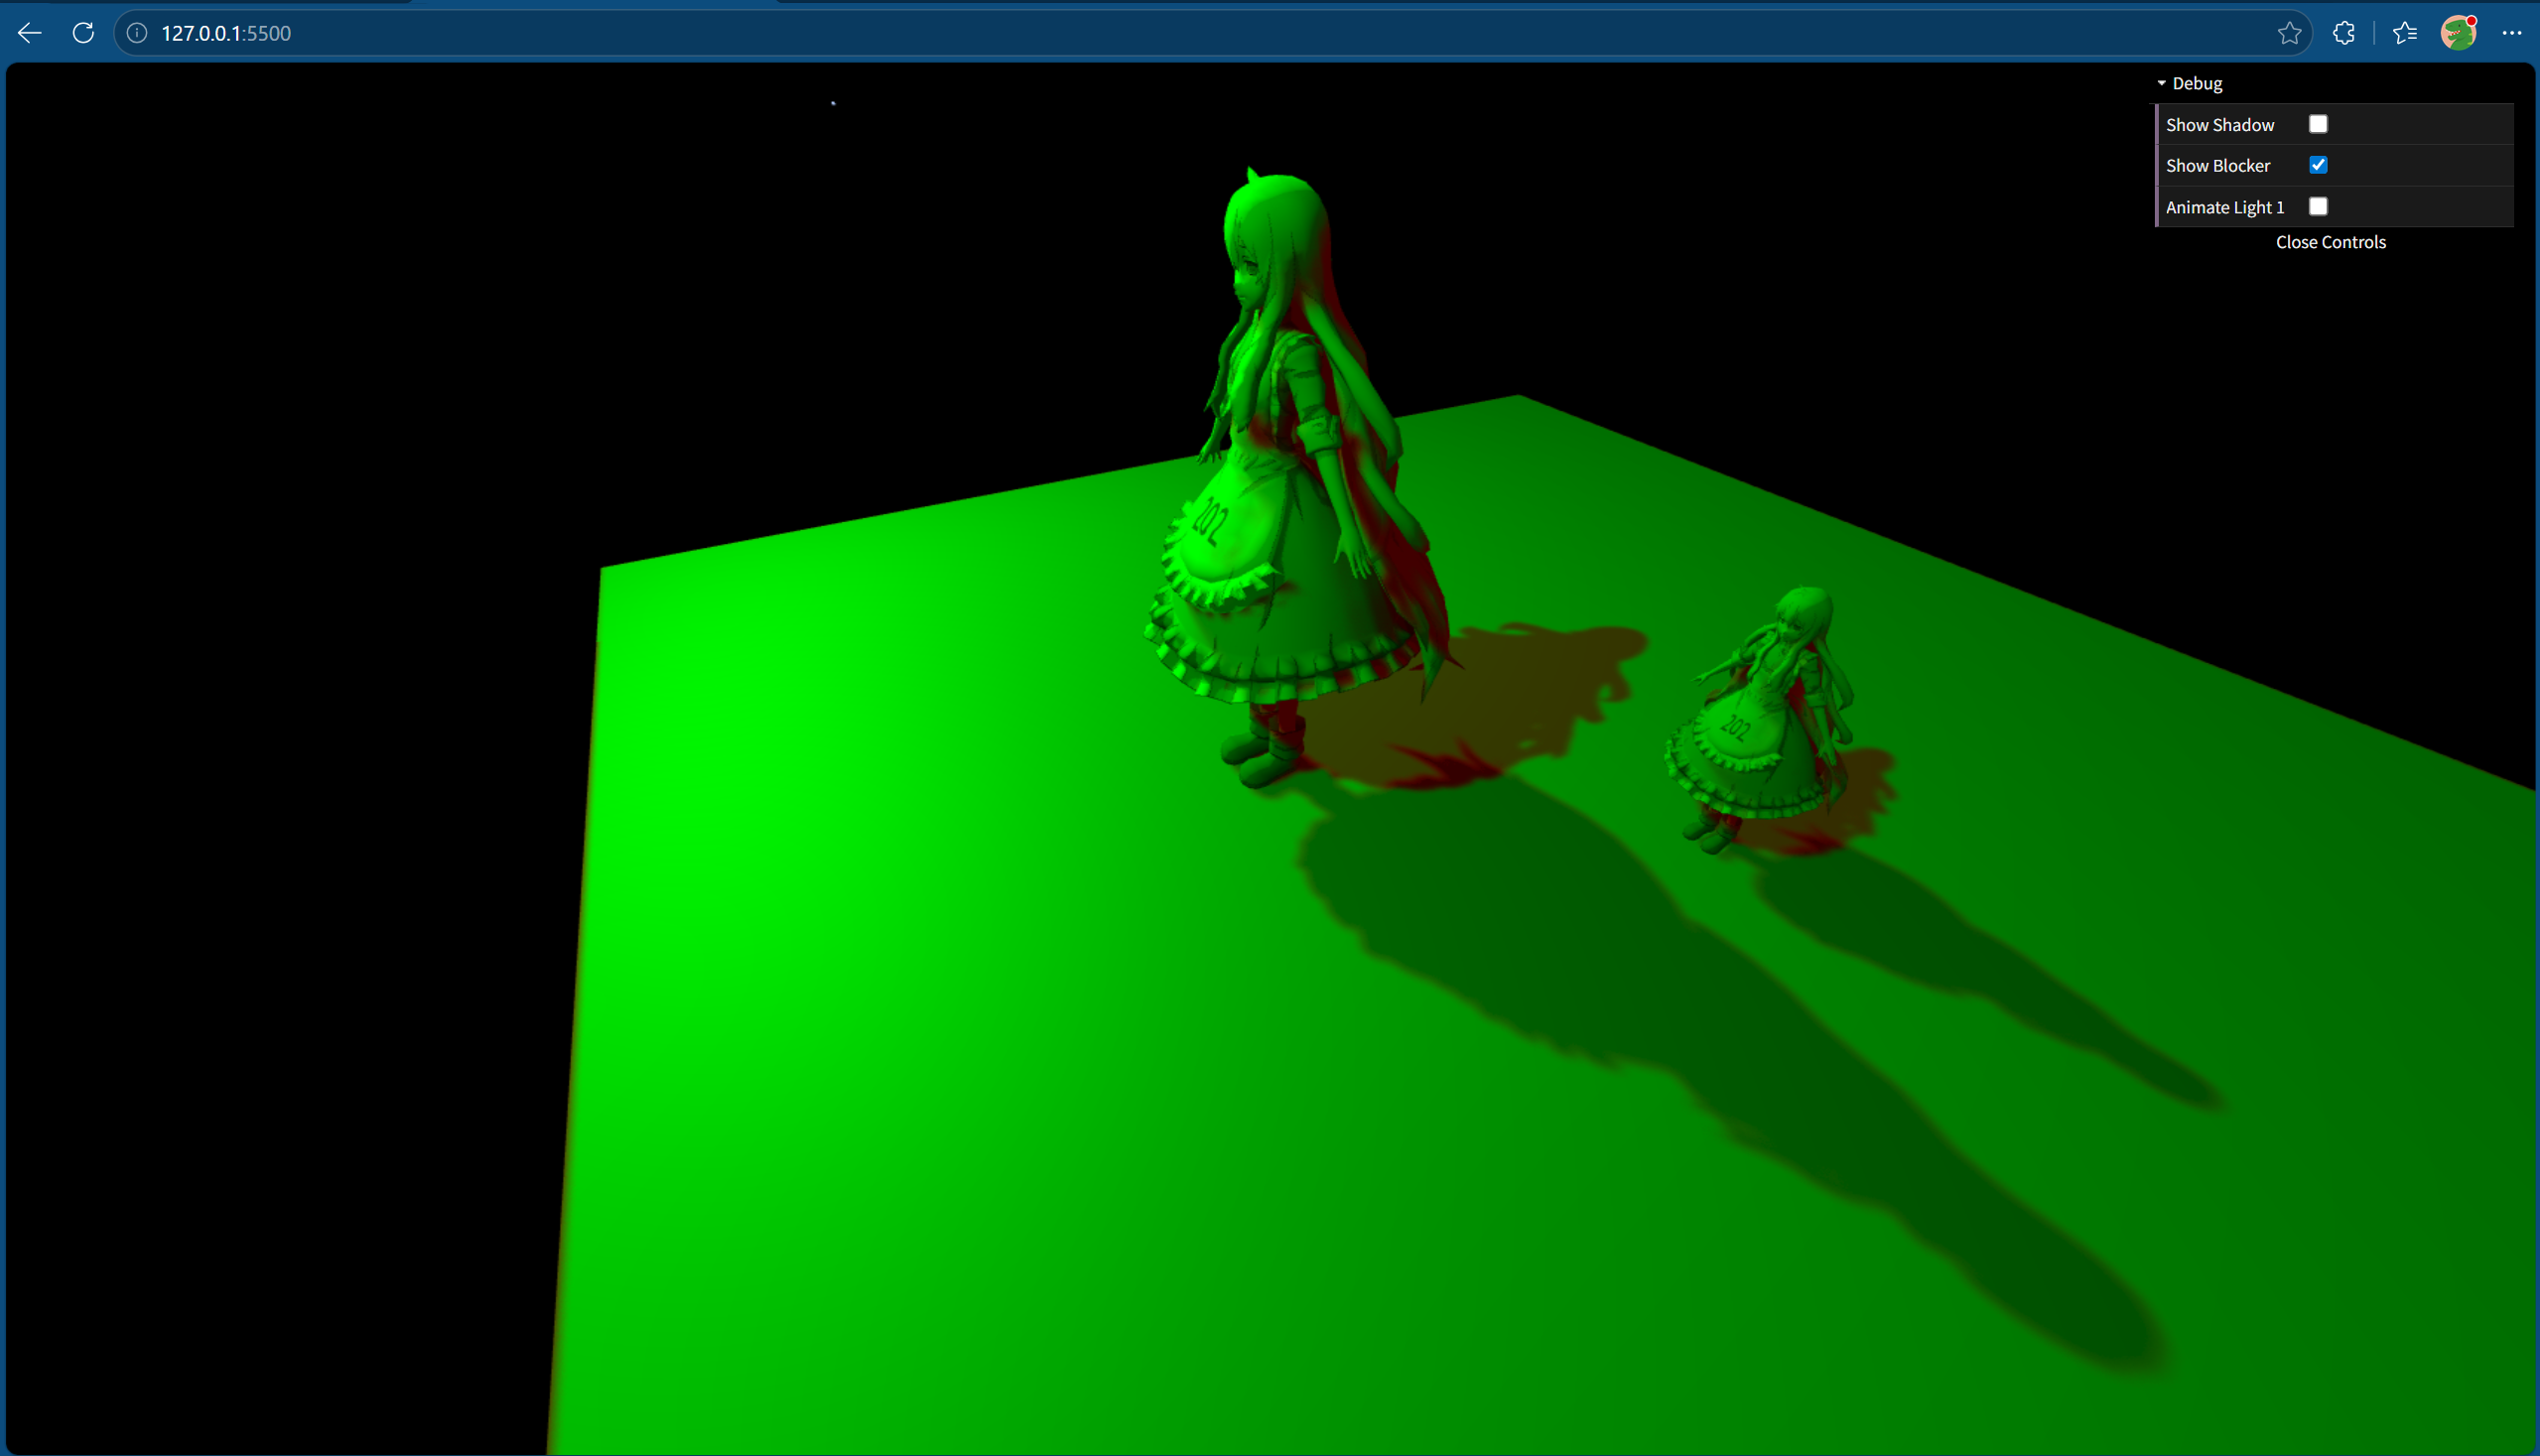
\includegraphics[width=\linewidth]{PCF_blocker_debug.png}\\[-1pt]
    \small PCF
  \end{minipage}
  \begin{minipage}{0.32\linewidth}
    \centering
    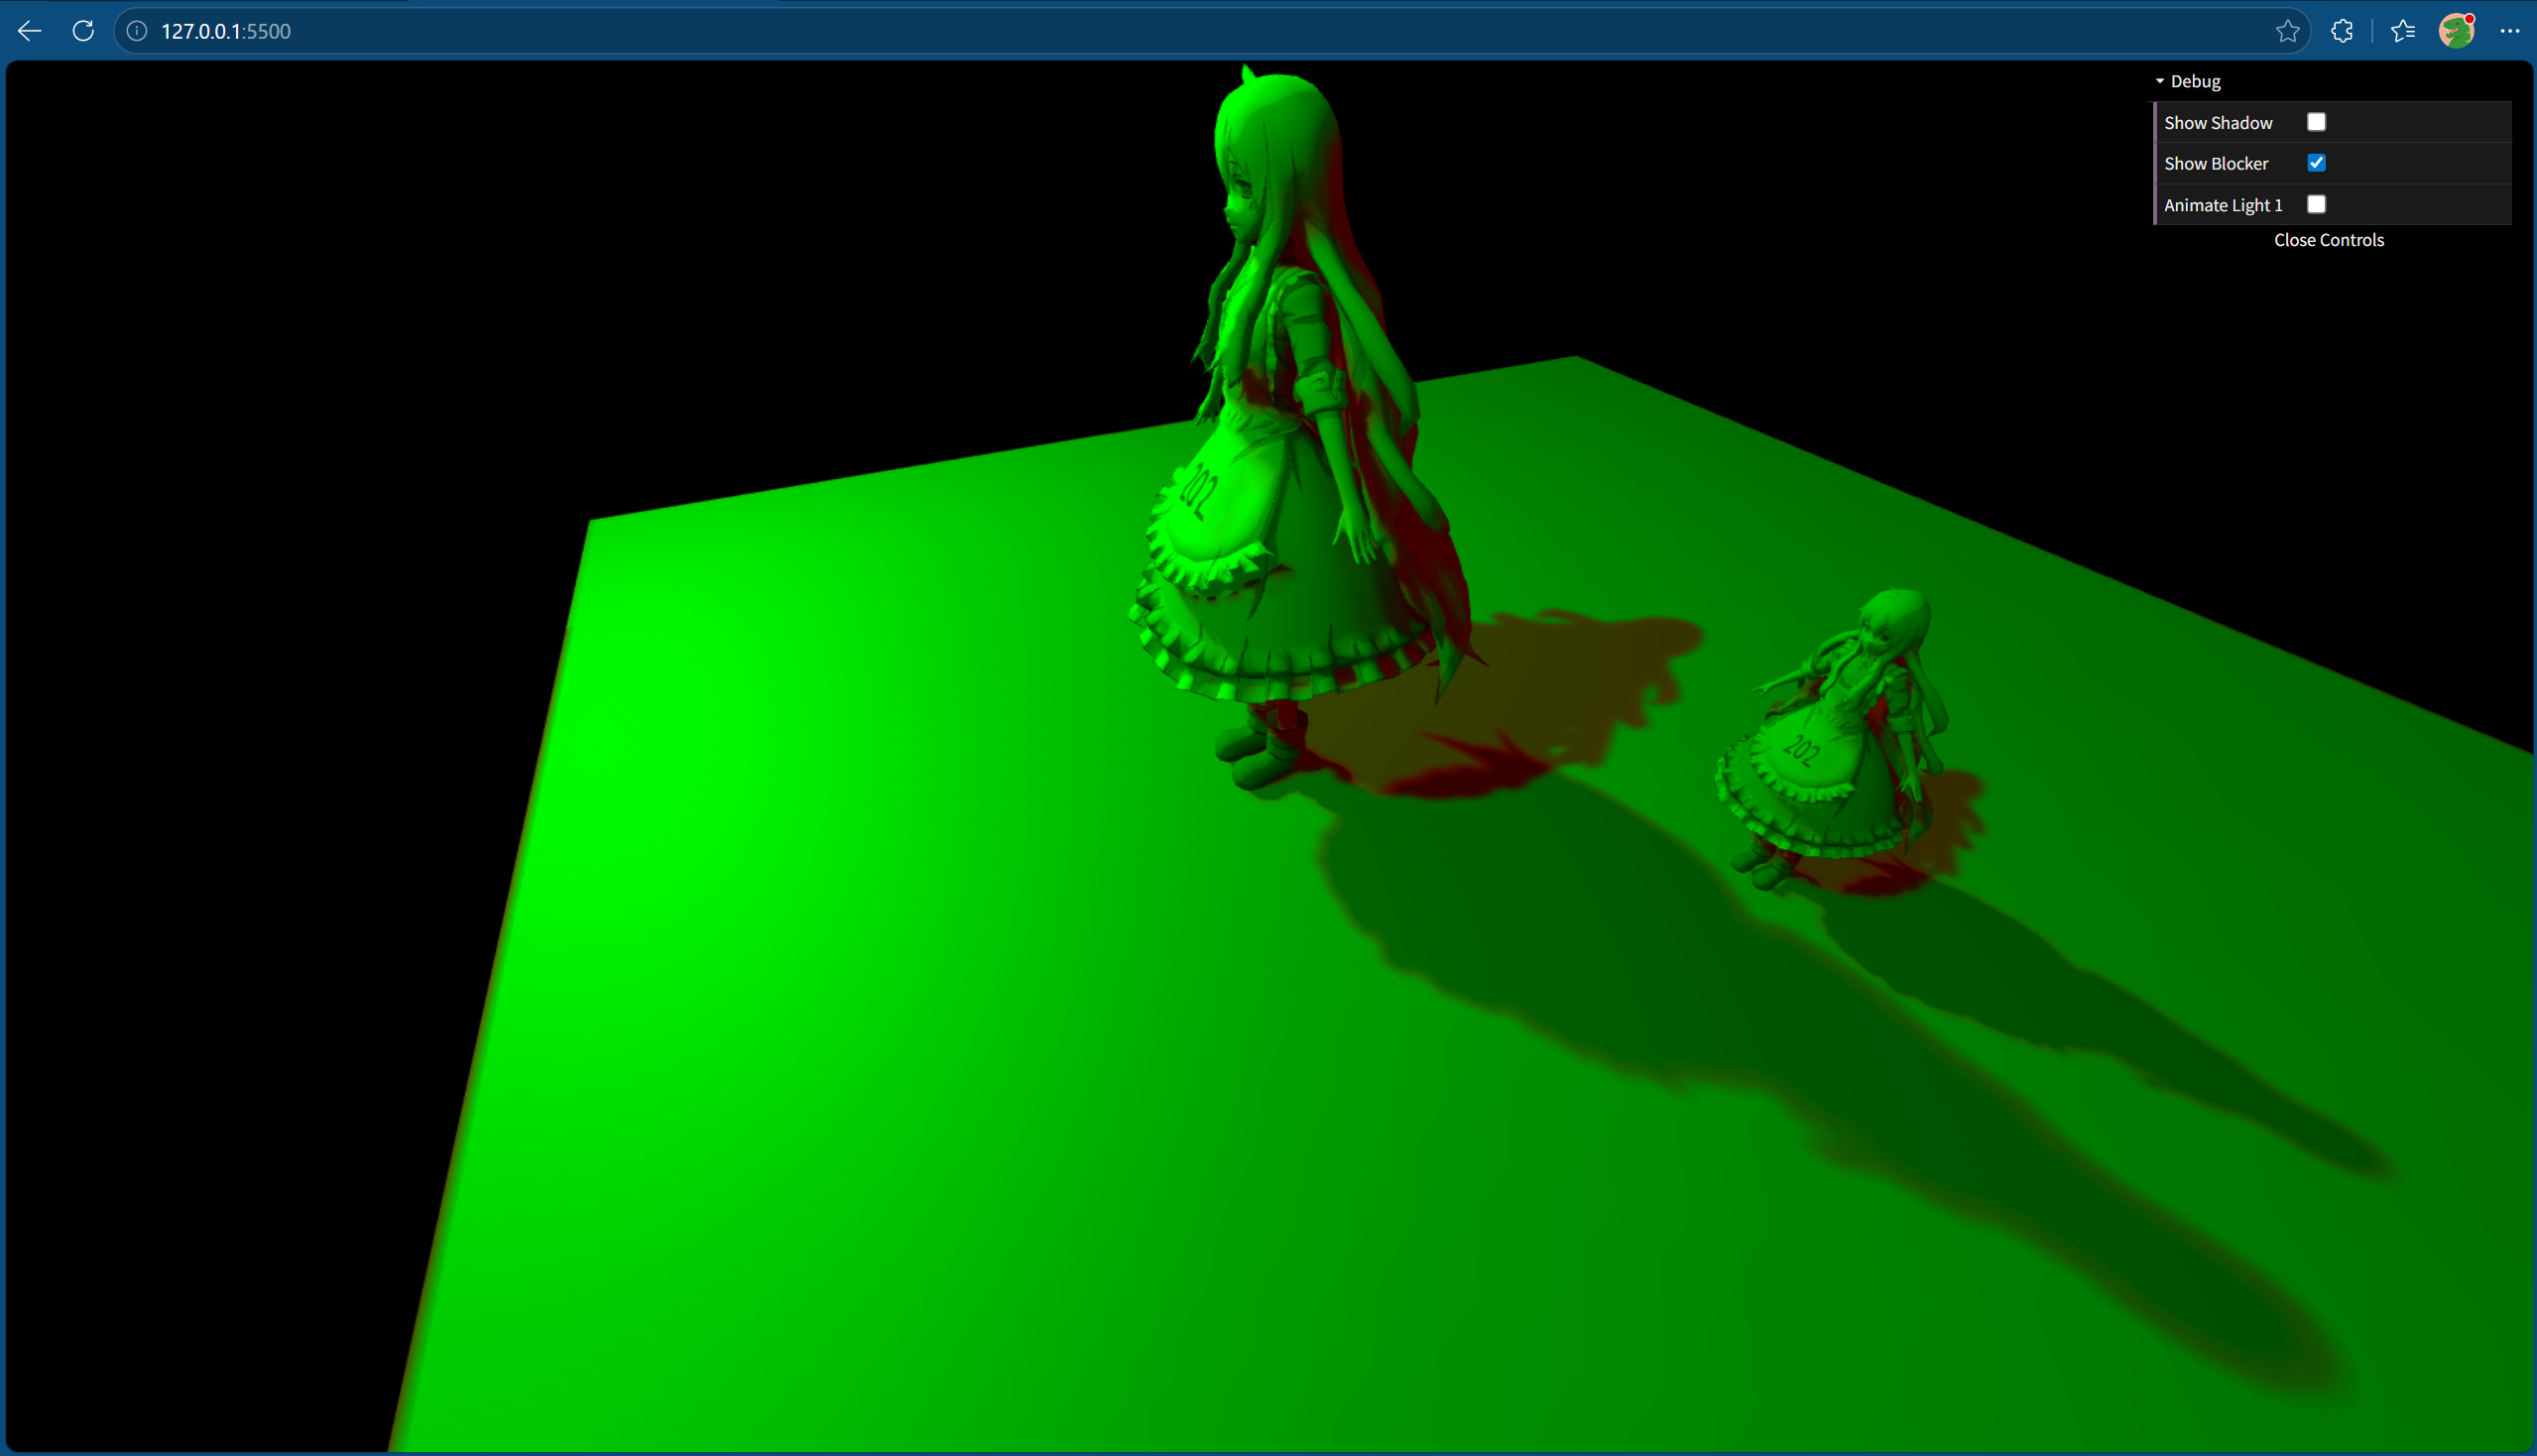
\includegraphics[width=\linewidth]{PCSS_blocker_debug.png}\\[-1pt]
    \small PCSS
  \end{minipage}
  \caption{三种显示模式下的 Blocker 搜索红绿色标可视化}
  \label{fig:blocker-debug}
\end{figure}

图 \ref{fig:blocker-debug} 的颜色分布应与几何遮挡关系一致，而不要求与最终阴影明暗完全相同：硬阴影和 PCF 仍按各自方式计算可见性，PCSS 则进一步使用 blocker 信息估计半影半径。

\subsection{多光源与移动光源结果}

固定暖色主光提供主要照明和阴影，轨道运动冷色光从另一个方向补充直接光照，并产生随时间变化的阴影方向。两个光源各自拥有 Shadow Map，直接光照通过 additive blending 线性叠加，环境光只在第一个 pass 中加入。图 \ref{fig:sm}、图 \ref{fig:pcf} 和图 \ref{fig:pcss} 均为双光源截图，因此出现两个方向的阴影是正确现象；移动光源某一时刻的效果也已经包含在这些截图中。

场景中的小 Mary 同时做圆形平动和绕 Y 轴自转，阴影实时跟随。在浏览器中打开后可通过 dat.gui 面板的 \texttt{Animate Model} 开关控制动画启停，便于截图时获得稳定位置。

\subsection{三种方法对比}

\begin{table}[htbp]
\centering
\caption{三种阴影方法的效果对比}
\begin{tabular}{p{0.16\linewidth}p{0.25\linewidth}p{0.27\linewidth}p{0.22\linewidth}}
\toprule
方法 & 优点 & 缺点 & 本项目表现 \\
\midrule
Shadow Map & 实现简单，阴影关系明确 & 边缘硬，锯齿明显 & 可验证遮挡关系正确 \\
PCF & 边缘平滑，实时性较好 & 滤波半径固定，缺少接触变化 & 适合稳定展示软阴影 \\
PCSS & 半影随深度变化，更接近面积光 & 开销较大，参数敏感 & 能表现接触硬、远处软 \\
\bottomrule
\end{tabular}
\end{table}

总体而言，硬阴影主要用于验证基础 Shadow Map 管线，PCF 解决了边界锯齿问题，PCSS 则进一步引入了深度相关的半影估计。由于当前项目运行在 WebGL1 环境，并使用 \(8192 \times 8192\) 的 Shadow Map 和多次采样，PCSS 的性能压力较高，刷新时可能受浏览器缓存、WebGL context 和 GPU 资源释放时序影响。因此实际截图时需要在切换 shader 后强制刷新，并等待资源加载完成。

\section{总结}

本文基于 WebGL 实现了实时阴影渲染中的三个核心任务及额外扩展。首先，通过 Two-Pass Shadow Map 建立了从光源视角记录深度、从相机视角进行遮挡判断的基础管线，实现了硬阴影。随后，在硬阴影基础上引入 Poisson 圆盘采样，实现了固定半径 PCF，使阴影边缘由二值跳变变为连续过渡。最后，实现 PCSS 中的 blocker search、平均遮挡物深度计算、半影大小估计和动态半径 PCF，使阴影能够呈现接触处较硬、远离遮挡物处较软的变化。在额外扩展中，项目还实现了调试可视化、双光源叠加和移动光源阴影。

在实现过程中，关键问题包括光源 MVP 的正确构造、Shadow Map 深度的打包与解包、采样越界处理、bias 参数选择以及性能与质量的平衡。最终实现中将 Shadow Map 纹理设置为 \texttt{CLAMP\_TO\_EDGE}，对 PCF/PCSS 采样点进行边界检查，并将阴影可见性只作用于直接光照项，从而避免环境光被整体压暗。

实验结果说明，Shadow Map、PCF 和 PCSS 三种方法均已在当前场景中完成，可通过 dat.gui 下拉菜单在运行时直接切换，无需修改 shader 或刷新页面。硬阴影用于展示基本遮挡关系，PCF 提供稳定的软化效果，PCSS 则进一步表现深度相关的软阴影特征。在此基础上，项目还实现了 Shadow Map 小窗、blocker 搜索区域可视化、多光源叠加、移动光源动画以及动态模型自转与平动。

\section{小组分工、电子签名与贡献百分比}

\begin{table}[htbp]
\centering
\caption{小组成员分工、电子签名与贡献百分比}
\small
\renewcommand{\arraystretch}{1.35}
\setlength{\tabcolsep}{4pt}
\begin{tabular}{@{}p{0.13\linewidth}p{0.51\linewidth}p{0.18\linewidth}p{0.10\linewidth}@{}}
\toprule
成员 & 主要分工 & 电子签名 & 贡献百分比 \\
\midrule
李志阳 &
负责 Shadow Map 硬阴影实现和扩展功能，包括 Shadow Map 可视化、blocker 可视化、动态光源与动态物体；参与答辩 PPT 制作和演示视频录制。 &
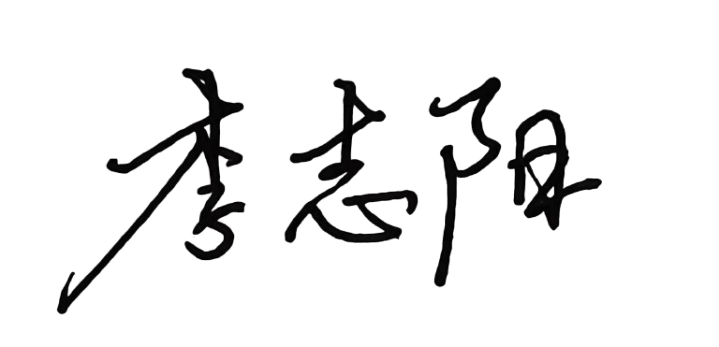
\includegraphics[height=1.05cm,keepaspectratio]{signature_lizhiyang.png} &
50\% \\
安燕杰 &
负责 PCF、PCSS 算法实现，PDF 报告撰写；参与答辩 PPT 制作。 &
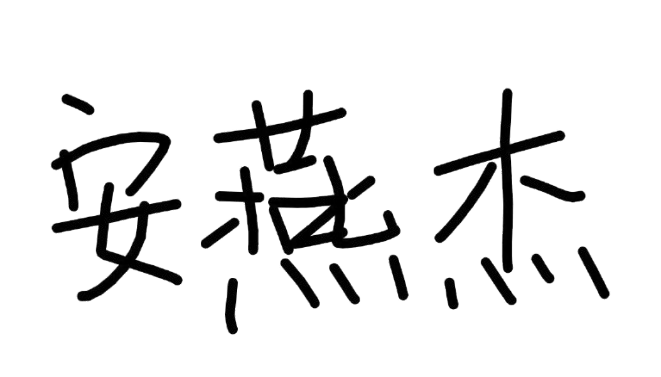
\includegraphics[height=1.05cm,keepaspectratio]{signature_anyanjie.png} &
50\% \\
\bottomrule
\end{tabular}
\end{table}

\end{document}
